% !TEX program = D:\LaTex\miktex\bin\x64\xelatex.exe
%==============================================================================
% LAPORAN PRAKTEK KERJA LAPANGAN (PKL)
% Program Studi Teknik Informatika, Institut Teknologi Sumatera
% Padanan LaTeX dari T1-Template_Laporan_PKL.docx
%
% Compile : xelatex main.tex  (jalankan 2x supaya Daftar Isi terisi sempurna)
% Font    : Times New Roman (otomatis fallback ke TeX Gyre Termes)
%==============================================================================

\documentclass[12pt,a4paper]{report}

%==============================================================================
% 1. KONFIGURASI TEMPLATE & CONSTRAINTS (CONFIG)
%==============================================================================
% Paket LaTeX, layout, styling, metadata, dan constraints disimpan terpisah di /config:
% - config/packages.tex   : Daftar package yang digunakan
% - config/layout.tex     : Pengaturan font, margin halaman, spasi, dan indentasi
% - config/styling.tex    : Format penomoran bab/section, caption, TOC, dan header-footer
% - config/metadata.tex   : Data judul, nama mahasiswa, NIM, instansi, & pembimbing
% - config/constraints.tex: Custom macro helper & ringkasan constraints resmi PKL ITERA

%==============================================================================
% CONFIG: MASTER LOADER
% Memuat seluruh paket, aturan tata letak, styling, metadata, dan constraints
%==============================================================================

%==============================================================================
% CONFIG: PAKET-PAKET LATEX (PACKAGES)
%==============================================================================

% Font dan tipografi
\usepackage{fontspec}

% Spasi dan geometri halaman
\usepackage{setspace}
\usepackage[a4paper,top=3cm,bottom=3cm,right=3cm,left=3.5cm,
            headheight=14pt,headsep=1.2cm,footskip=1.5cm]{geometry}

% Grafis dan tabel
\usepackage{graphicx}
\usepackage{float}
\usepackage{array}

% Format paragraf, list, dan penomoran
\usepackage{indentfirst}  % Paragraf pertama setelah heading tetap menjorok 1,27 cm
\usepackage{enumitem}

% Tata letak header, footer, heading, dan daftar isi
\usepackage{fancyhdr}
\usepackage{titlesec}
\usepackage{tocloft}
\usepackage{caption}

% Hyperlink
\usepackage[hidelinks]{hyperref}

%==============================================================================
% CONFIG: LAYOUT, TIPOGRAFI, DAN SPASI
%==============================================================================

% Font: Times New Roman (fallback ke TeX Gyre Termes bila font sistem belum terpasang)
\IfFontExistsTF{Times New Roman}{%
  \setmainfont{Times New Roman}%
}{%
  \setmainfont{TeX Gyre Termes}%
}

% Tipografi: Times New Roman 12 pt, rata kiri-kanan, spasi 1,5 (setara Microsoft Word)
%   Word "1.5 lines" TNR 12 pt = 20,7 pt  ->  skala 1,43 dari baselineskip LaTeX
%   Word "single"     TNR 12 pt = 13,8 pt  ->  skala 0,952
\newcommand{\spasisatu}{\setstretch{0.952}}
\newcommand{\spasisetengah}{\setstretch{1.43}}
\AtBeginDocument{\spasisetengah}

% Indentasi & spasi antar paragraf
\setlength{\parindent}{1.27cm}   % First-line indent 720 twips (1,27 cm)
\setlength{\parskip}{10pt}       % Spacing after paragraf 200 twips (10 pt)
\setlength{\emergencystretch}{2em}

% Label penamaan bahasa Indonesia
\renewcommand{\figurename}{Gambar}
\renewcommand{\tablename}{Tabel}
\renewcommand{\contentsname}{Daftar Isi}

%==============================================================================
% CONFIG: STYLING (HEADING, PENOMORAN, HEADER-FOOTER, TOC, CAPTION, LIST)
%==============================================================================

%------------------------------------------------------------------------------
% PENOMORAN: Bab (I, II, ...), subbab 1.1., sub-subbab 1.1.1.
%------------------------------------------------------------------------------
\renewcommand{\thechapter}{\Roman{chapter}}
\renewcommand{\thesection}{\arabic{chapter}.\arabic{section}}
\renewcommand{\thesubsection}{\arabic{chapter}.\arabic{section}.\arabic{subsection}}
\renewcommand{\thefigure}{\arabic{chapter}.\arabic{figure}}
\renewcommand{\thetable}{\arabic{chapter}.\arabic{table}}
\setcounter{secnumdepth}{2}
\setcounter{tocdepth}{2}

%------------------------------------------------------------------------------
% HEADING FORMAT
%   Heading 1 (Chapter): rata tengah, tebal, "Bab I" lalu nama bab di baris baru
%   Heading 2 (Section): tebal, nomor 1.1.
%   Heading 3 (Subsection): tebal, nomor 1.1.1.
%------------------------------------------------------------------------------
\titleformat{\chapter}[display]
  {\normalfont\bfseries\centering\spasisetengah}
  {Bab \thechapter}{0pt}{}
\titlespacing*{\chapter}{0pt}{0pt}{12pt}

\titleformat{\section}[hang]
  {\normalfont\bfseries\spasisetengah}
  {\makebox[1.27cm][l]{\thesection.}}{0pt}{}
\titlespacing*{\section}{0pt}{3pt}{3pt}

\titleformat{\subsection}[hang]
  {\normalfont\bfseries\spasisetengah}
  {\makebox[1.27cm][l]{\thesubsection.}}{0pt}{}
\titlespacing*{\subsection}{0pt}{12pt}{3pt}

% Judul halaman khusus (misal: lembar pengesahan, daftar lain-lain)
\newcommand{\judulhal}[1]{%
  \begingroup\centering\bfseries #1\par\endgroup\vspace{3pt}}

%------------------------------------------------------------------------------
% NOMOR HALAMAN (PAGINATION)
%   Halaman pertama bab/lampiran : bottom center
%   Halaman berikutnya           : top right
%------------------------------------------------------------------------------
\fancypagestyle{halamanisi}{%
  \fancyhf{}%
  \renewcommand{\headrulewidth}{0pt}%
  \renewcommand{\footrulewidth}{0pt}%
  \fancyhead[R]{\thepage}%
}

\fancypagestyle{plain}{%
  \fancyhf{}%
  \renewcommand{\headrulewidth}{0pt}%
  \renewcommand{\footrulewidth}{0pt}%
  \fancyfoot[C]{\thepage}%
}

\pagestyle{halamanisi}

%------------------------------------------------------------------------------
% CAPTION: Tabel di atas tabel, Gambar di bawah gambar, format <bab>.<urutan>
%------------------------------------------------------------------------------
\captionsetup{labelsep=period,justification=centering,singlelinecheck=true,
              font=normalsize,labelfont=normalfont}
\captionsetup[table]{position=above,skip=6pt}
\captionsetup[figure]{position=below,skip=6pt}

%------------------------------------------------------------------------------
% DAFTAR ISI (TOC) DENGAN TOCLOFT
%------------------------------------------------------------------------------
\renewcommand{\cfttoctitlefont}{\bfseries}
\renewcommand{\cftaftertoctitle}{}
\renewcommand{\cftchapfont}{\bfseries}
\renewcommand{\cftchappagefont}{\bfseries}
\renewcommand{\cftchappresnum}{Bab }
\renewcommand{\cftdotsep}{0.6}   % Titik leader rapat
\renewcommand{\cftchapleader}{\bfseries\cftdotfill{\cftdotsep}}
\setlength{\cftchapnumwidth}{3.4em}
\setlength{\cftbeforechapskip}{3pt}
\setlength{\cftbeforesecskip}{3pt}
\setlength{\cftbeforesubsecskip}{3pt}
\setlength{\cftsecindent}{0.635cm}
\setlength{\cftsecnumwidth}{1.0cm}
\renewcommand{\cftsecaftersnum}{.}
\setlength{\cftsubsecindent}{1.27cm}
\setlength{\cftsubsecnumwidth}{1.3cm}
\renewcommand{\cftsubsecaftersnum}{.}

%------------------------------------------------------------------------------
% LIST / PENOMORAN ITEM
%------------------------------------------------------------------------------
\setlist{nosep}
\setlist[enumerate]{leftmargin=1.27cm,labelwidth=0.635cm,labelsep=0pt,align=left,
                    itemsep=0pt,topsep=0pt,parsep=0pt}

%==============================================================================
% CONFIG: METADATA & DATA ISIAN LAPORAN PKL
% Ubah data di bawah ini sesuai dengan identitas dan instansi Anda.
%==============================================================================

%------------------------------------------------------------------------------
% 1. IDENTITAS LAPORAN & TOPIK
% [Constraint]: Judul cover huruf kapital (ALL CAPS), bold, maksimal 3 baris.
%------------------------------------------------------------------------------
\newcommand{\JudulCover}{<JUDUL TUGAS AKHIR (DITULIS DALAM HURUF KAPITAL; TIMES NEW ROMAN; 16 PT; DICETAK TEBAL / BOLD; TIDAK MELEBIHI DARI 3 BARIS>}
\newcommand{\TopikKP}{<TOPIK KERJA PRAKTEK>}
\newcommand{\TahunLaporan}{2026}

%------------------------------------------------------------------------------
% 2. IDENTITAS MAHASISWA
%------------------------------------------------------------------------------
\newcommand{\NamaMhs}{Nama mahasiswa}
\newcommand{\NIM}{NIM}

%------------------------------------------------------------------------------
% 3. IDENTITAS INSTANSI / TEMPAT PKL
%------------------------------------------------------------------------------
\newcommand{\NamaPerusahaan}{<Nama Perusahaan>}
\newcommand{\KotaInstansi}{<Kota>}
\newcommand{\TanggalInstansi}{<Tanggal>}

%------------------------------------------------------------------------------
% 4. PEMBIMBING PROGRAM STUDI (ITERA)
%------------------------------------------------------------------------------
\newcommand{\NamaPembimbingProdi}{<Nama Pembimbing>}
\newcommand{\NIPPembimbingProdi}{123456789}
\newcommand{\TanggalPengesahanProdi}{……}

%------------------------------------------------------------------------------
% 5. PEMBIMBING & PENANGGUNG JAWAB INSTANSI
%------------------------------------------------------------------------------
\newcommand{\JabatanPembimbingInstansi}{<Jabatan Penanggung jawab/ Pembimbing di tempat kerja>}
\newcommand{\NamaPembimbingInstansi}{Nama Penanggung Jawab di instansi}
\newcommand{\NoPegawaiPembimbingInstansi}{<Nomor Induk Pegawai/Nomor Pegawai>}

% Penandatangan kedua pada Lampiran A TOR (Atasan di Instansi)
\newcommand{\NamaAtasanInstansi}{Nama Atasan/Jabatan}
\newcommand{\NoPegawaiAtasanInstansi}{Nomor Pegawai}

%==============================================================================
% CONFIG: CONSTRAINTS, RULES, & MACROS HELPER
% Program Studi Teknik Informatika, Institut Teknologi Sumatera
%==============================================================================

%------------------------------------------------------------------------------
% MACRO / HELPER PERINTAH FORMAT
%------------------------------------------------------------------------------

% Petunjuk template (cetak miring / tebal miring)
\newcommand{\pet}[1]{\textit{#1}}
\newcommand{\petb}[1]{\textbf{\textit{#1}}}

% Butir bab pada Sistematika Penulisan (Bab I)
% Format: bullet + judul bab tebal, lalu deskripsi isi miring
\newcommand{\butirbab}[2]{%
  \begin{itemize}[leftmargin=0.635cm,labelwidth=0.635cm,labelsep=0pt,align=left,
                  label=\textbullet,itemsep=0pt,topsep=0pt,parsep=0pt]
    \item \textbf{#1}
  \end{itemize}
  \noindent\pet{#2}\par}

% Pengaturan awal halaman Lampiran
% Penomoran: <Huruf>-1, <Huruf>-2, dll. (contoh: A-1, B-1)
% Gambar/Tabel: <Huruf>.1, <Huruf>.2, dll. (contoh: Gambar D.1.)
\newcommand{\mulailampiran}[1]{%
  \clearpage
  \renewcommand{\thepage}{#1-\arabic{page}}%
  \setcounter{page}{1}%
  \renewcommand{\thefigure}{#1.\arabic{figure}}%
  \renewcommand{\thetable}{#1.\arabic{table}}%
  \setcounter{figure}{0}\setcounter{table}{0}%
  \thispagestyle{plain}%
}

% Judul halaman Lampiran
\newcommand{\judullampiran}[2]{%
  \addcontentsline{toc}{chapter}{Lampiran #1. #2}%
  \begingroup\centering\bfseries Lampiran #1. #2\par\endgroup\vspace{12pt}}

%------------------------------------------------------------------------------
% RINGKASAN ATURAN & CONSTRAINTS TEMPLATE LAPORAN PKL (REFERENSI RESMI)
%------------------------------------------------------------------------------
% 1. TIPOGRAFI & MARGIN:
%    - Font Utama   : Times New Roman, 12 pt.
%    - Margin Kertas: Top 3 cm, Bottom 3 cm, Right 3 cm, Left 3.5 cm (A4).
%    - Spasi        : 1.5 spasi (skala baselineskip 1.43, setara Microsoft Word).
%    - Indentasi    : First-line indent 1.27 cm (720 twips).
%    - Par-spacing  : Space after paragraph 10 pt (200 twips).
%
% 2. COVER (Halaman Sampul):
%    - Judul TA/PKL : HURUF KAPITAL (ALL CAPS), Bold, 16 pt, MAKSIMAL 3 BARIS.
%    - Logo         : Wajib memuat Logo Resmi ITERA.
%
% 3. LEMBAR PENGESAHAN:
%    - Lembar Pengesahan Prodi ITERA: tanda tangan Dosen Pembimbing PKL & NIP.
%    - Lembar Pengesahan Instansi   : tanda tangan Pembimbing Lapangan/Penanggung Jawab, cap instansi.
%
% 4. ABSTRAK:
%    - Bahasa       : Bahasa Indonesia baku.
%    - Panjang      : Maksimal 250 kata, WAJIB tepat dalam 1 halaman.
%    - Isi wajib    : Ringkasan lingkup PKL (termasuk nama perusahaan), masalah instansi,
%                     pelaksanaan/proses, kesimpulan umum, dan kata kunci (keywords).
%
% 5. DAFTAR GAMBAR & DAFTAR TABEL:
%    - Jika hanya ada 1 gambar atau 1 tabel di seluruh laporan, TIDAK PERLU dibuatkan daftar.
%    - Jika ada, masing-masing diletakkan pada halaman terpisah.
%
% 6. BAB ISI:
%    - Bab I        : Latar Belakang DILARANG membahas alasan kurikuler mata kuliah PKL.
%                     Fokus pada problem-solving informatika di instansi.
%                     Rumusan Masalah WAJIB dijawab tuntas pada Bab VI Kesimpulan.
%    - Bab II       : Wajib menyertakan Gambar Logo Perusahaan.
%                     Diagram Struktur Organisasi WAJIB diberi highlight (shading/garis putus)
%                     pada posisi/divisi tim PKL. Durasi PKL wajib 25 s.d. 40 hari kerja.
%    - Bab III      : DILARANG mengutip dari Wikipedia, koran, portal berita non-ilmiah.
%                     Wajib dari jurnal, buku, prosiding ilmiah.
%    - Bab IV       : Menguraikan analisis masalah, alur penyelesaian (flowchart), gambaran sistem,
%                     alat & bahan, serta metodologi pengembangan.
%    - Bab V        : Menyajikan hasil implementasi dan pengujian seluruh fitur dari Bab IV,
%                     serta evaluasi/analisis presentasi di instansi.
%    - Bab VI       : Kesimpulan wajib menjawab semua rumusan masalah & tujuan. Saran pengembangan.
%
% 7. REFERENSI (DAFTAR PUSTAKA):
%    - Gaya sitasi  : Gaya IEEE (nomor siku [1], [2], dst.).
%    - Pengurutan   : Diurutkan secara alfabetis berdasarkan nama pengarang.
%    - Kuota Sumber : MINIMAL 10 referensi, MAKSIMAL 3 referensi website (sisanya jurnal/buku).
%
% 8. LAMPIRAN:
%    - Lampiran A   : TOR (Term of Reference) - Wajib, ditandatangani 3 pihak.
%    - Lampiran B   : Log Sheet (Form KP2) bertanda tangan & cap resmi instansi.
%    - Lampiran C   : Dokumen Teknik (SRS, manual book, source code). Jika confidential,
%                     wajib diganti surat pernyataan resmi bertanda tangan dari perusahaan.
%    - Lampiran D   : Dokumentasi Kegiatan - Wajib ada dokumentasi foto per minggunya.
%------------------------------------------------------------------------------



%==============================================================================
% 2. DOKUMEN UTAMA
%==============================================================================
\begin{document}

%------------------------------------------------------------------------------
% BAGIAN AWAL (FRONT MATTER)
%------------------------------------------------------------------------------
%==============================================================================
% HALAMAN SAMPUL (COVER)
% Sesuai panduan T1-Template Laporan PKL ITERA
% [Constraint]:
% - Judul Tugas Akhir: HURUF KAPITAL (ALL CAPS), font 16 pt, tebal, maks 3 baris
% - Tanpa nomor halaman
%==============================================================================
\begin{titlepage}
  \thispagestyle{empty}
  \centering
  \spasisatu
  {\bfseries\fontsize{16}{19}\selectfont
   LAPORAN PRAKTEK KERJA LAPANGAN\par
   \vspace{12pt}
   \JudulCover\par
   \vspace{12pt}
   DI \NamaPerusahaan\par}
  \vspace{40pt}
  Diajukan untuk memenuhi persyaratan kelulusan\par
  \vspace{6pt}
  Matakuliah IF4004 Praktek Kerja Lapangan\par
  \vspace{20pt}
  Oleh:\par
  \vspace{6pt}
  \NamaMhs\par
  \vspace{3pt}
  \NIM\par
  \vspace{36pt}
  
\includegraphics[width=4.31cm,height=5.22cm]{figure/logo-itera.png}\par
  \vspace{36pt}
  {\bfseries\fontsize{14}{17}\selectfont
   PROGRAM STUDI TEKNIK INFORMATIKA\par
   \vspace{3pt}
   INSTITUT TEKNOLOGI SUMATERA\par
   \vspace{3pt}
   \TahunLaporan\par}
\end{titlepage}

%==============================================================================
% LEMBAR PENGESAHAN PROGRAM STUDI TEKNIK INFORMATIKA ITERA
%==============================================================================
\pagenumbering{arabic}
\setcounter{page}{1}
\pagestyle{plain}
\thispagestyle{plain}

\begin{center}
\spasisetengah
\judulhal{Lembar Pengesahan Program Studi Teknik Informatika}
\vspace{12pt}

\textbf{\TopikKP}\par
\vspace{12pt}
\textbf{Di \NamaPerusahaan}\par
\vspace{6pt}
Oleh:\par
\vspace{6pt}
\NamaMhs\par
\NIM\par
\vspace{36pt}
disetujui dan disahkan sebagai\par
Laporan Praktek Kerja Lapangan\par
\end{center}

\vspace{6pt}
\noindent\begin{minipage}{0.62\textwidth}\raggedright\parindent=0pt\parskip=0pt
Lampung Selatan, \TanggalPengesahanProdi\par
Pembimbing Praktek Kerja Lapangan Program Studi Teknik Informatika ITERA\par
\pet{<ttd digital/basah sesuai kesepakatan>}\par
\vspace{1.2cm}
\NamaPembimbingProdi\par
NIP: \NIPPembimbingProdi\par
\end{minipage}

%==============================================================================
% LEMBAR PENGESAHAN INSTANSI / PERUSAHAAN
%==============================================================================
\clearpage
\thispagestyle{plain}

\begin{center}
\spasisetengah
\judulhal{Lembar Pengesahan}
\vspace{12pt}

\textbf{\TopikKP}\par
\vspace{12pt}
\textbf{Di \NamaPerusahaan}\par
\vspace{6pt}
oleh :\par
\vspace{6pt}
\NamaMhs\par
\NIM\par
\vspace{36pt}
disetujui dan disahkan sebagai\par
Laporan Praktek Kerja Lapangan\par
\end{center}

\vspace{6pt}
\noindent\begin{minipage}{0.62\textwidth}\raggedright\parindent=0pt\parskip=0pt
\KotaInstansi, \TanggalInstansi\par
\JabatanPembimbingInstansi\par
\pet{<ttd digital/ langsung/cap basah sesuai ketentuan dari instansi>}\par
\vspace{1.2cm}
\NamaPembimbingInstansi\par
\NoPegawaiPembimbingInstansi\par
\end{minipage}

%==============================================================================
% ABSTRAK
% [Constraints]:
% - Maksimal 250 kata & wajib tepat dalam 1 halaman
% - Bahasa Indonesia yang baik dan benar
% - Memuat: lingkup PKL (termasuk nama perusahaan), masalah instansi, pelaksanaan/hasil,
%   kesimpulan umum, dan kata kunci
%==============================================================================
\chapter*{ABSTRAK}
\addcontentsline{toc}{chapter}{ABSTRAK}

\noindent\pet{Tuliskan ringkasan laporan Kerja Praktek, yang merupakan ringkasan dari lingkup kerja praktek (termasuk nama perusahaan, penjelasan singkat terkait permasalahan di instansi, pelaksanaan kerja praktek (proses dan pencapaian hasil), kesimpulan umum mengenai kerja praktek yang telah dilakukan dan kata kunci, dalam Bahasa Indonesia. (\petb{dituliskan dalam maksimal 250 kata \& hanya dalam 1 halaman}).}

\noindent\pet{Kata kunci: …}

%==============================================================================
% KATA PENGANTAR
%==============================================================================
\chapter*{Kata Pengantar}
\addcontentsline{toc}{chapter}{Kata Pengantar}

\noindent\pet{Tuliskan rasa terimakasih kepada siapa saja yang terkait dengan Praktek Kerja Lapangan ini. Penulisan Kata Pengantar dengan bahasa Indonesia yang baik dan benar.}

%==============================================================================
% DAFTAR ISI
%==============================================================================
\clearpage
{\spasisatu
\setlength{\parskip}{0pt}
\renewcommand{\cfttoctitlefont}{\hfill\bfseries}
\renewcommand{\cftaftertoctitle}{\hfill}
\tableofcontents}

%==============================================================================
% DAFTAR LAIN-LAIN
% [Constraints]:
% - Dapat ditambahkan: daftar tabel, daftar gambar, daftar algoritma, daftar singkatan, simbol, dll.
% - Jika hanya terdapat 1 gambar atau 1 tabel di seluruh laporan, TIDAK PERLU dibuatkan daftar.
% - Setiap daftar diletakkan pada halaman terpisah.
%==============================================================================
\clearpage
\thispagestyle{plain}
\judulhal{<Daftar lain-lain>}

\noindent\pet{Dapat ditambahkan berbagai daftar yang dibutuhkan seperti daftar tabel, daftar gambar, daftar algoritma, daftar padanan istilah, daftar singkatan, daftar istilah, daftar simbol. Khusus untuk daftar pustaka (Referensi), dapat diletakkan setelah bab Kesimpulan, sebelum lampiran. Jika hanya terdapat satu gambar atau satu tabel, maka tidak perlu dibuat daftar gambar atau daftar tabel. Setiap daftar, misal daftar gambar, daftar tabel, daftar istilah dan singkatan, semuanya diletakkan pada halaman terpisah.}


%------------------------------------------------------------------------------
% BAGIAN ISI UTAMA (MAIN BODY CHAPTERS)
%------------------------------------------------------------------------------
%==============================================================================
% BAB I: PENDAHULUAN
%==============================================================================
\pagestyle{halamanisi}
\chapter{Pendahuluan}

\section{Latar Belakang}
Salah satu indikator utama dalam menilai tingkat kesejahteraan suatu bangsa adalah kesehatan masyarakat. Pemerintah Indonesia telah mengupayakan berbagai langkah untuk mendukung terwujudnya kesehatan masyarakat yang optimal, salah satunya melalui penyelenggaraan layanan rumah sakit. Di samping itu, pemerintah juga menghadirkan Program Jaminan Kesehatan Nasional (JKN) sebagai bentuk jaminan atas akses layanan kesehatan yang efektif dan efisien bagi seluruh lapisan masyarakat \cite{10}.

Program JKN diselenggarakan melalui skema asuransi sosial, dengan tujuan meringankan beban finansial masyarakat yang timbul akibat kebutuhan layanan kesehatan \cite{10}. Penggantian biaya atas layanan kesehatan yang telah diterima masyarakat dilakukan melalui mekanisme pengajuan klaim BPJS oleh pihak rumah sakit \cite{1}. Proses pengajuan klaim tersebut mengharuskan terpenuhinya sejumlah persyaratan, baik dari sisi kelengkapan administrasi maupun ketepatan kode diagnosis dan tindakan medis yang diberikan \cite{1}. Persyaratan ini menjadi acuan untuk memastikan keabsahan proses pembiayaan sekaligus mencegah terjadinya penolakan klaim oleh pihak BPJS Kesehatan. Apabila persyaratan administrasi belum terpenuhi atau terdapat ketidaksesuaian kode diagnosis dan tindakan, maka klaim akan berstatus pending \cite{10}, \cite{14}.

Ketika klaim BPJS berstatus pending, berkas yang bermasalah akan dikembalikan kepada rumah sakit untuk dilakukan peninjauan ulang \cite{14}. Kondisi pending claim ini umumnya disebabkan oleh sejumlah faktor, di antaranya keterbatasan sumber daya manusia \cite{10}, \cite{14}, kesalahan dalam proses koding \cite{10}, \cite{16}, serta ketidaklengkapan dokumen pendukung klaim \cite{10}, \cite{16}. Permasalahan tersebut berdampak langsung pada terganggunya arus kas rumah sakit, yang pada gilirannya dapat menghambat pembayaran gaji pegawai, kewajiban kepada pemasok, dan alokasi biaya pemeliharaan fasilitas rumah sakit \cite{10}, \cite{14}.

Kondisi ini menunjukkan perlunya analisis lebih mendalam serta langkah penanganan yang tepat guna mengidentifikasi akar permasalahan dan menekan potensi terjadinya pending klaim BPJS Kesehatan.

\section{Rumusan Masalah}
Dari latar belakang yang telah dijelaskan sebelumnya, maka rumusan masalah pada Praktek Kerja Lapangan ini adalah sebagai berikut:
\begin{enumerate}
    \item Bagaimana proses alur administrasi serta faktor-faktor penyebab terjadinya pending claim pada pengajuan klaim BPJS Kesehatan dapat dianalisis?
    \item Bagaimana rekomendasi sistem yang mampu meminimalisir risiko terjadinya pending claim pada pengajuan klaim BPJS Kesehatan dapat dirancang?
\end{enumerate}

\section{Tujuan}
Adapun tujuan dari Praktek Kerja Lapangan ini adalah sebagai berikut:
\begin{enumerate}
    \item Menganalisis alur administrasi, faktor-faktor penyebab, dan potensi terjadinya pending claim pada pengajuan klaim BPJS Kesehatan.
    \item Merancang rekomendasi sistem untuk meminimalisir risiko terjadinya pending claim pada pengajuan klaim BPJS Kesehatan.
\end{enumerate}

\section{Manfaat}
\subsection{Bagi Mahasiswa}
\begin{enumerate}
    \item Memperoleh wadah untuk mengimplementasikan ilmu yang telah diperoleh selama menempuh perkuliahan.
    \item Memperoleh gambaran mengenai kondisi lingkungan kerja pada instansi/perusahaan tempat pelaksanaan PKL.
    \item Menumbuhkan sikap tanggung jawab serta kedisiplinan pada diri mahasiswa.
    \item Membentuk dan mengasah sikap maupun pola pikir profesional sebagai bekal sebelum memasuki dunia kerja yang sesungguhnya.
\end{enumerate}

\subsection{Bagi Prodi Teknik Informatika}
\begin{enumerate}
    \item Menjadi bahan masukan dalam evaluasi bidang akademik guna peningkatan dan pengembangan mutu pendidikan.
    \item Mencetak lulusan Program Studi Teknik Informatika yang memiliki kompetensi sesuai dengan kebutuhan dunia kerja.
\end{enumerate}

\subsection{Bagi Instansi}
\begin{enumerate}
    \item Berkontribusi dalam mendukung terciptanya sumber daya manusia yang kompeten di dunia kerja.
    \item Menjalin pertukaran informasi di bidang teknologi antara pihak instansi dengan mahasiswa pelaksana PKL.
\end{enumerate}

\section{Ruang Lingkup}
Adapun ruang lingkup analisis dan penanganan dari permasalahan yang diangkat pada laporan ini adalah sebagai berikut.
\begin{enumerate}
    \item Pengamatan dan analisis dititikberatkan pada alur administrasi dokumen pengajuan klaim BPJS Kesehatan.
    \item Laporan ini terbatas pada tahap identifikasi masalah administratif dan perancangan rekomendasi sistem, serta tidak mencakup tahap implementasi secara penuh maupun pengujian langsung pada lingkungan rumah sakit.
    \item Data dan alur administrasi yang dianalisis mengacu pada hasil studi literatur serta arahan yang diberikan oleh pembimbing lapangan perusahaan.
\end{enumerate}

\section{Sistematika Penulisan}
Kegiatan yang dilakukan untuk menyelesaikan Praktik Kerja Lapangan ini adalah identifikasi masalah, menentukan tujuan, melakukan studi literatur, pengumpulan data, analisis serta evaluasi. Seluruh kegiatan tersebut didokumentasikan dalam sistematika penulisan sebagai berikut.

\butirbab{Bab I Pendahuluan}{Bab ini memuat latar belakang pelaksanaan kegiatan, rumusan masalah, tujuan, manfaat, ruang lingkup beserta batasannya, dan sistematika penulisan laporan PKL.}
\butirbab{Bab II Gambaran Umum Instansi}{Bab ini berfungsi sebagai pembuka yang memperkenalkan instansi tempat PKL dilaksanakan. Isinya mencakup sejarah singkat, visi dan misi, serta struktur organisasi instansi.}
\butirbab{Bab III Landasan Teori}{Bab ini menguraikan teori-teori yang menjadi dasar penyusunan laporan PKL. Teori tersebut dirujuk dari buku, jurnal, regulasi, maupun standar yang relevan.}
\butirbab{Bab IV Metode Penelitian}{Bab ini menjabarkan pelaksanaan PKL, meliputi gambaran permasalahan yang dihadapi, tahapan penyelesaiannya, serta metode yang dipakai.}
\butirbab{Bab V Hasil Implementasi}{Bab ini menyajikan hasil analisis dan perancangan, serta pembahasan mengenai sejauh mana tujuan tercapai, dengan merujuk pada teori dan penelitian terdahulu.}
\butirbab{Bab VI Kesimpulan dan Saran}{Bab ini berisi kesimpulan sebagai jawaban atas rumusan masalah yang telah ditetapkan, serta saran-saran yang berkaitan dengan isi laporan.}

%==============================================================================
% BAB II: GAMBARAN UMUM INSTANSI
%==============================================================================
\chapter{Gambaran Umum Instansi}

\section{Profil Organisasi}
\begin{figure}[H]
  \centering
  
\includegraphics[width=6cm]{figure/logo-perusahaan-karla.png}
  \caption{Logo Perusahaan Karla Bionics}
\end{figure}

P.T. Bangga Teknologi Produktif (Karla Bionics) merupakan sebuah startup bisnis sosial di bidang teknologi yang didirikan di Bandung pada tahun 2019. Berawal dari hasil riset dan pengabdian masyarakat oleh akademisi Institut Teknologi Bandung (ITB), perusahaan ini memiliki visi untuk mengembangkan teknologi asistif yang inklusif, terjangkau, dan berpusat pada kebutuhan pengguna disabilitas. Karla Bionic memposisikan diri sebagai penggerak inovasi sosial. Pendekatan ini diwujudkan dengan menekankan pentingnya keberlanjutan dan dialog dengan para pihak yang berkepentingan, memastikan setiap solusi yang dihasilkan berakar pada kebutuhan nyata masyarakat sehingga menghasilkan manfaat yang jelas, tidak fokus pada laba atau keuntungan.

Raga Arm adalah produk unggulan dari Karla Bionics, yaitu, sebuah lengan prostetik dengan 2 varian, yaitu, mekanik dan elektrik. Produk ini dirancang dengan menggabungkan fungsi teknis dengan estetika untuk meningkatkan kepercayaan diri pengguna. Dengan mengusung konsep bionic aesthetic, Raga Arm telah diakui di tingkat internasional melalui partisipasinya dalam ajang Cybathlon Challenges 2022 dan 2023.

Karla Bionic menjalankan 2 peran sebagai pengembang teknologi layak pakai sekaligus penggerak inovasi sosial yang memberdayakan komunitas disabilitas. Identitas unik yang menyeimbangkan aspek teknis, sosial, dan keberlanjutan sebagai landasan bagi setiap produk yang dikembangkan oleh perusahaan.

\section{Visi dan Misi Organisasi}
\subsection{Visi Karla Bionics}
Menjadi usaha rintisan bisnis sosial berbasis teknologi terdepan dalam meningkatkan kualitas hidup para pemangku kepentingan secara berkelanjutan.

\subsection{Misi Karla Bionics}
\begin{enumerate}
    \item Mengembangkan teknologi tepat guna yang dilandaskan pada kebutuhan pemangku kepentingan.
    \item Mengembangkan program inovasi sosial yang berakar pada kebutuhan pemangku kepentingan.
    \item Melaksanakan pengembangan teknologi dan program sosial untuk saling mendukung, melalui proses dialog dengan para pemangku kepentingan.
\end{enumerate}

\section{Struktur Organisasi}
PT. Bangga Teknologi Produktif (Karla Bionic) dipimpin oleh seorang Chief Executive Officer (CEO) dengan dua posisi di bawahnya, yaitu, Chief Product Officer (CPO) dengan tanggung jawab mengembangkan produk, kemudian Chief Social Innovation Officer (CSIO) yang memiliki fokus pada inovasi sosial. Di bawah CPO dan CSIO terdapat tim-tim yang memiliki tugas untuk melakukan riset dan pengembangan sesuai bidang masing-masing.

\begin{figure}[H]
  \centering
  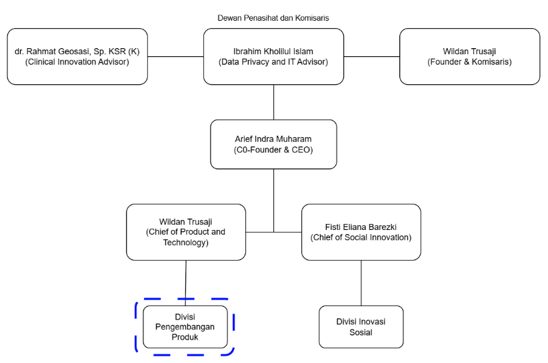
\includegraphics[width=12.36cm]{figure/struktur-organisasi-karla.png}
  \caption{Struktur PT Bangga Teknologi Produktif}
\end{figure}

Pada saat pelaksanaan PKL, tim PKL ditempatkan di Divisi Pengembangan Produk yang berfokus pada penelitian dan pengembangan.

\section{Deskripsi Pekerjaan}
Dalam pelaksanaan Praktek Kerja Lapangan (PKL) yang telah dilaksanakan, penulis bertugas sebagai Backend Engineer yang berfokus pada pengembangan logika sistem, database, dan Dokumentasi API agar decision support system untuk koding dalam klaim BPJS dapat disimulasikan.

Rincian kegiatan yang dilakukan selama periode PKL adalah sebagai berikut.

\noindent\textbf{Fase 1 : Analisis Permasalahan}\\
Dalam fase ini, tim PKL menganalisis dan mencari informasi terkait permasalahan yang diberikan oleh perusahan.

\noindent\textbf{Fase 2 : Analisis Solusi dari Permasalahan}\\
Dalam fase ini, tim PKL menganalisis solusi yang dapat mengatasi permasalahan yang telah disepakati bersama dengan pembimbing lapangan.

\noindent\textbf{Fase 3 : Pengembangan Frontend}\\
Dalam fase ini, penulis mengembangkan backend yang disesuaikan dengan rencana pengembangan sistem.

\noindent\textbf{Fase 4 : Integrasi Frontend Dengan Backend}\\
Dalam fase ini, tim PKL mengintegrasikan Frontend dan Backend yang telah dikembangkan serta memperbaiki kekurangan sistem yang muncul setelah integrasi.

\section{Jadwal Kerja}
\begin{table}[H]
  \centering
  \caption{Jadwal Kerja}
  \begin{tabular}{|l|c|c|c|p{5.5cm}|}
    \hline
    \textbf{Hari} & \textbf{Jam Masuk} & \textbf{Jam Istirahat} & \textbf{Jam Pulang} & \textbf{Keterangan} \\
    \hline
    Senin  & 09.00 & 11.30-13.00 & 17.00 & Kegiatan rutin di Kantor \\ \hline
    Selasa & 09.00 & 11.30-13.00 & 17.00 & Kegiatan rutin di Kantor \\ \hline
    Rabu   & 09.00 & 11.30-13.00 & 17.00 & Kegiatan rutin di Kantor \\ \hline
    Kamis  & 09.00 & 11.30-13.00 & 17.00 & Kegiatan rutin di Kantor, Evaluasi Mingguan \\ \hline
    Jumat  & 09.00 & 11.30-13.00 & 17.00 & Kegiatan rutin di Kantor \\ \hline
  \end{tabular}
\end{table}

%==============================================================================
% BAB III: LANDASAN TEORI
% [Constraints]:
% - Sumber wajib ilmiah: buku, jurnal, prosiding, skripsi/TA, web resmi terpercaya
% - DILARANG menggunakan Wikipedia, blogspot, koran, atau portal berita non-ilmiah
%==============================================================================
\chapter{Landasan Teori}

\pet{Pada bagian ini dijelaskan mengenai konsep dan dasar teori yang digunakan dalam implementasi sistem, aplikasi, atau prototype yang dikembangkan.}

\section{Dasar Teori}
\pet{Berisi teori/konsep yang berkaitan/digunakan dalam kerja praktek. Gunakanlah data melalui buku/jurnal referensi, publikasi tugas akhir, penelitian, buku, dan informasi web yang dapat dipertanggungjawabkan, \petb{hindari penggunaan dasar teori melalui tautan Wikipedia, surat kabar, atau portal berita, yang dapat memiliki isi yang tidak bersifat fakta.}}

\section{Teori I}
\pet{Deskripsikan mengenai teori/konsep yang berkaitan/digunakan/menjadi acuan dalam penelitian. Kemudian berikan pembahasan sederhana mengenai penggunaannya di dalam laporan PKL yang Anda kerjakan.}

\section{Teori II}
\pet{Deskripsikan mengenai teori / konsep yang berkaitan / digunakan / menjadi acuan dalam penelitian. Kemudian berikan pembahasan sederhana mengenai penggunaannya di dalam tugas akhir yang Anda kerjakan.}

\subsection{Sub Teori I}
\pet{Sub Teori dapat dituliskan dengan level penomoran 3 \& style “Heading 3”}

%==============================================================================
% BAB IV: METODE PENELITIAN
% [Catatan]: Rincian subbab dapat disesuaikan dengan output pekerjaan PKL Anda.
%==============================================================================
\chapter{Metode Penelitian}

\pet{Pada bagian ini dijelaskan mengenai pelaksanaan PKL meliputi deskripsi persoalan, alur proses penyelesaian, gambaran umum, dan metodologi pengembangan dari perangkat lunak, keras, sistem, dan prototype yang dikembangkan atau dibangun. Adapun rincian dari substansi pada Bab IV adalah sebagai subbab berikut, tetapi subbab dapat disesuaikan kembali dengan output yang anda kerjakan pada tempat kerja praktek anda.}

\pet{Caption tabel dan gambar ditulis dengan format <bab>.<urutan tabel/gambar>. Caption tabel berada di atas tabel, sedangkan caption gambar berada di bawah gambar.}

\begin{table}[H]
  \centering
  \caption{Contoh \textit{caption} tabel}
  \spasisatu
  \setlength{\arrayrulewidth}{1pt}
  \begin{tabular}{|p{4.35cm}|p{4.35cm}|p{4.35cm}|}
    \hline
    \rule{0pt}{14pt} & & \\
    \hline
    \rule{0pt}{14pt} & & \\
    \hline
    \rule{0pt}{14pt} & & \\
    \hline
  \end{tabular}
\end{table}

\begin{figure}[H]
  \centering
  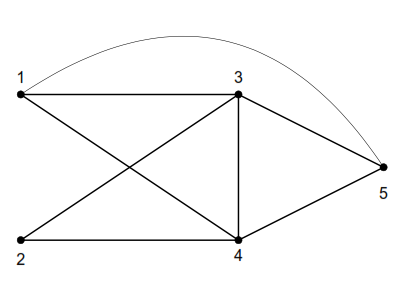
\includegraphics[width=5.95cm,height=4.47cm]{figure/contoh-gambar.png}
  \caption{Contoh \textit{caption} gambar}
\end{figure}

\section{Analisis Permasalahan}
\pet{Tuliskan analisis dari persoalan yang harus diselesaikan dalam kerja praktek, termasuk usulan solusi untuk persoalan tersebut. Sesuaikan dengan latar belakang persoalan, deskripsi persoalan, batasan yang harus diselesaikan dalam PKL, teknologi terkait yang mendukung solusi dari persoalan, dan hal lain yang terkait dengan persoalan PKL.}

\section{Alur Penyelesaian}
\pet{Tuliskan alur penyelesaian PKL anda dengan detail, dari mulai observasi, identifikasi masalah, perumusan masalah, pemilihan metode, implementasi, pengujian, dan penarikan kesimpulan. Supaya lebih tergambar dengan jelas, bisa dengan menggunakan \textit{flowchart}.}

\section{Gambaran Umum Sistem/Aplikasi/Prototype}
\pet{Gambarkanlah secara umum terkait arsitektur sistem/aplikasi/prototype yang anda kembangkan. Dapat menggunakan diagram atau gambar sebagai pembantu.}

\section{Alat dan Bahan}
\pet{Uraikan spesifikasi dari alat dan bahan yang digunakan untuk mendukung pengembangan sistem atau prototype.}

\subsection{Alat}
\pet{Alat yang digunakan untuk melakukan pengembangan sistem atau prototype, dapat berupa komputer, PC, Arduino, raspberry, dsb.}

\begin{enumerate}
  \item Notebook, dengan spesifikasi…
  \item Smartphone, dengan spesifikasi…
  \item Software XYZ
\end{enumerate}

\subsection{Bahan}
\pet{Bahan yang digunakan/diperlukan untuk melakukan pengembangan sistem atau prototype, dapat berupa:}

\begin{enumerate}
  \item Dataset pihak pertama yang diperoleh secara langsung, melalui izin instansi.
  \item Dataset pihak lain yang diperoleh dengan izin atau dalam lisensi yang diizinkan untuk digunakan secara langsung.
  \item Dataset pihak pertama yang disusun sendiri melalui kuesioner, observasi, atau interview.
\end{enumerate}

\section{Metodologi Pengembangan}
\pet{Uraikan secara detail terkait dengan metodologi yang anda gunakan untuk membangun dan mengembangkan sistem atau prototype, termasuk alur pengembangan, desain/diagram sistem, rencana pengembangan, cara pengumpulan data, \textit{low/high fidelity}, dsb.}

%==============================================================================
% BAB V: HASIL IMPLEMENTASI
%==============================================================================
\chapter{Hasil Implementasi}

\pet{Tuliskan bagaimana hasil dari implementasi dari perangkat lunak, perangkat keras, sistem, atau prototype yang anda kembangkan. Sertakan juga lingkup implementasi anda dalam merancang perangkat lunak, perangkat keras, sistem, atau prototype.}

\section{Hasil Implementasi}
\pet{Tuliskan hasil dari proses pengembangan. Tuliskan hasil pengujian dari semua fitur-fitur yang sudah dirancang pada bab IV berdasarkan metodologi yang digunakan selama menyelesaikan dan mengembangkan perangkat lunak, keras, sistem, atau prototype.}

\section{Evaluasi dan Analisis}
\pet{Tuliskan evaluasi dan analisis sederhana, dapat berupa tabel, visualisasi data, atau narasi, berdasarkan hasil implementasi dan pengujian yang anda dapatkan. Evaluasi dapat menceritakan hasil presentasi terhadap instansi bersangkutan, termasuk \textit{stakeholder} yang terlibat dan tanggal presentasi.}

%==============================================================================
% BAB VI: KESIMPULAN DAN SARAN
% [Constraints]:
% - Kesimpulan WAJIB menjawab seluruh butir Rumusan Masalah & sesuai Tujuan di Bab I.
%==============================================================================
\chapter{Kesimpulan dan Saran}

\pet{Tuliskan apa yang perlu disampaikan sebagai penutup berupa kesimpulan dan saran PKL.}

\section{Kesimpulan}
\pet{Tuliskan kesimpulan baik mengenai proses pelaksanaan PKL maupun mengenai substansi yang dikerjakan selama PKL. Kesimpulan harus menjawab semua poin Rumusan Masalah \& sesuai dengan Tujuan yang terdapat dalam Bab I.}

\section{Saran}
\pet{Tuliskan saran terhadap penelitian (berdasarkan observasi \& analisis hasil) untuk kedepannya. Saran juga dapat berkaitan mengenai proses pelaksanaan PKL selama bekerja di instansi, agar dapat menjadi lebih baik kedepannya.}


%------------------------------------------------------------------------------
% BAGIAN AKHIR & LAMPIRAN (BACK MATTER & APPENDICES)
%------------------------------------------------------------------------------
%==============================================================================
% REFERENSI (DAFTAR PUSTAKA)
% [Constraints]:
% - Gaya Sitasi: IEEE (nomor dalam kurung siku [1], [2], dst.)
% - Urutan: Alfabetis (abjad) berdasarkan nama pengarang
% - Kuota: Minimal 10 referensi (website maksimal 3, sisanya jurnal/buku/prosiding)
%==============================================================================
\chapter*{Referensi}
\addcontentsline{toc}{chapter}{Referensi}

\pet{Tuliskan berbagai referensi yang digunakan dalam laporan PKL terurut abjad berdasar nama pengarang dan beri nomor mulai dari [1], dengan gaya IEEE.}

\pet{Referensi yang digunakan \petb{minimal 10} (diperbolehkan mengambil referensi dari website, tetapi tidak boleh lebih dari 3).}

% Silakan buka komentar (uncomment) pada blok thebibliography di bawah ini untuk mengisi:
% Format IEEE:
% 1. Jurnal: Inisial. Nama, "Judul artikel," Nama Jurnal, vol. x, no. x, pp. xx-xx, Tahun.
% 2. Buku: Inisial. Nama, Judul Buku, Edisi ke-x. Kota Terbit: Penerbit, Tahun.
% 3. Prosiding: Inisial. Nama, "Judul makalah," dalam Nama Konferensi, Kota, Tahun, pp. xx-xx.
% 4. Website: Inisial. Nama / Organisasi, "Judul halaman web," URL, diakses Tanggal-Bulan-Tahun.

\begin{thebibliography}{99}
  \bibitem{ref1}
  A. B. Penulis, ``Penerapan Sistem Informasi Manajemen pada Rumah Sakit,'' \textit{Jurnal Rekayasa Sistem dan Teknologi Informasi}, vol. 5, no. 2, pp. 101--110, 2024.

  \bibitem{ref2}
  C. D. Author and E. F. Coauthor, \textit{Systems Analysis and Design Methods}, 7th ed. New York: McGraw-Hill, 2021.
\end{thebibliography}

%==============================================================================
% LAMPIRAN A: TOR (TERM OF REFERENCE)
% [Constraints]:
% - Wajib bagi seluruh mahasiswa PKL, disusun pada awal pelaksanaan PKL.
% - Wajib ditandatangani 3 pihak: Mahasiswa, Pembimbing Lapangan, dan Atasan Instansi.
% - Penomoran halaman dimulai dari A-1, A-2, dst.
%==============================================================================
\mulailampiran{A}

\pet{Penulisan halaman untuk setiap lampiran sama dengan format penulisan halaman untuk setiap bab, contoh untuk Lampiran A, halaman berawal dari A-1, A-2, dst. Posisi nomor halaman pada halaman pertama ditulis pada bottom center, untuk halaman berikutnya adalah top right. Hal ini juga berlaku untuk nomor halaman pada bab isi.}

\judullampiran{A}{TOR (Term of Reference)}

\noindent\pet{Lampiran A bersifat wajib untuk mahasiswa yang melakukan KP. TOR berisi \textit{job description} Mahasiswa PKL dan target PKL yang telah disepakati bersama antara Mahasiswa PKL dan Perusahaan. TOR ini dibuat pada awal pelaksanaan PKL dan ditandatangani oleh pihak Mahasiswa PKL dan Perusahaan. Pembimbing dari Program Studi akan membantu mahasiswa melaksanakan PKL dan menyusun laporan PKL sesuai TOR yang telah disepakati.}

\noindent\textbf{Penjabaran}

{\parskip=0pt
\noindent\pet{Latar Belakang}\par
\noindent\pet{Tujuan Pekerjaan}\par
\noindent\pet{Lingkup Pekerjaan}\par
\noindent\pet{Metodologi}\par
\noindent\pet{Hasil Pekerjaan}\par
\noindent\pet{Jadwal Kerja}\par
\noindent\pet{Lain-lain}\par
\noindent\pet{Kerahasiaan dan Perlindungan Informasi}\par}

\clearpage
\begin{center}
\pet{Terms of reference} ini telah dibaca dan disetujui oleh:\par
\vspace{12pt}
Pihak Mahasiswa\par
\vspace{12pt}
\pet{TTD}\par
\vspace{12pt}
\NamaMhs\par
\NIM\par
\vspace{12pt}
Pihak Instansi\par
\vspace{12pt}
\pet{TTD \& cap}\par
\vspace{12pt}
\NamaPembimbingInstansi\par
\NoPegawaiPembimbingInstansi\par
\vspace{12pt}
Pihak Instansi\par
\vspace{12pt}
\pet{TTD \& cap}\par
\vspace{12pt}
\NamaAtasanInstansi\par
\NoPegawaiAtasanInstansi\par
\end{center}

%==============================================================================
% LAMPIRAN B: LOG SHEET
% [Constraints]:
% - Berisi Form Presensi & Logsheet (KP2) yang sudah bertanda tangan dan cap resmi instansi.
% - Jumlah hari kerja: 25 - 40 hari kerja.
%==============================================================================
\mulailampiran{B}
\judullampiran{B}{Log Sheet}

\pet{Log Sheet dapat melampirkan \petb{Form Presensi \& Logsheet} (KP2) yang sudah ditandatangani \& dicap oleh instansi. Tabel Log Sheet dapat menyesuaikan dengan jumlah hari kerja.}

%==============================================================================
% LAMPIRAN C: DOKUMEN TEKNIK
% [Constraints]:
% - Berisi SRS, Manual Book, Source Code, Skema Basis Data, dsb.
% - Wajib ada, KECUALI jika instansi menyatakan dokumen bersifat confidential.
% - Jika confidential, WAJIB diganti surat pernyataan resmi bertanda tangan dari perusahaan.
%==============================================================================
\mulailampiran{C}
\judullampiran{C}{Dokumen Teknik}

\pet{Mahasiswa PKL dapat melampirkan berbagai dokumen teknik yang merupakan hasil pelaksanaan PKL, contoh \petb{Software Requirement Specification (SRS), Manual Book, Kode Program, dll}. Lampiran ini wajib ada, kecuali bagi perusahaan yang menyatakan bahwa dokumen teknis terkait PKL bersifat \textit{confidential}. Jika dokumen teknis bersifat \textit{confidential}, maka lampiran ini diganti dengan lampiran surat pernyataan dari perusahaan dan ditandatangani oleh pembimbing di perusahaan bahwa \petb{dokumen teknis terkait PKL bersifat confidential.}}

%==============================================================================
% LAMPIRAN D: DOKUMENTASI KEGIATAN
% [Constraints]:
% - Foto kegiatan pelaksanaan PKL (offline maupun online/remote).
% - Dokumentasi visual WAJIB ADA PER MINGGUNYA.
% - Penomoran gambar: Gambar D.1., Gambar D.2., dst.
%==============================================================================
\mulailampiran{D}
\judullampiran{D}{Dokumentasi Kegiatan}

\pet{Berisi foto-foto kegiatan pelaksanaan PKL. Foto tersebut dapat dalam bentuk foto kegiatan langsung (\textit{offline}) atau \textit{screenshot} kegiatan (jika pelaksanaan PKL secara \textit{remote/online}) atau kombinasi keduanya. Dokumentasi juga dapat dalam bentuk video, berupa link Youtube.}

\petb{Foto dokumentasi wajib ada perminggunya.}

\begin{enumerate}[leftmargin=0.635cm,labelwidth=0.635cm,labelsep=0pt,align=left]
  \item \textbf{Minggu 1 (<Tanggal>-<Bulan>-<Tahun>)}
\end{enumerate}

\begin{figure}[H]
  \centering
  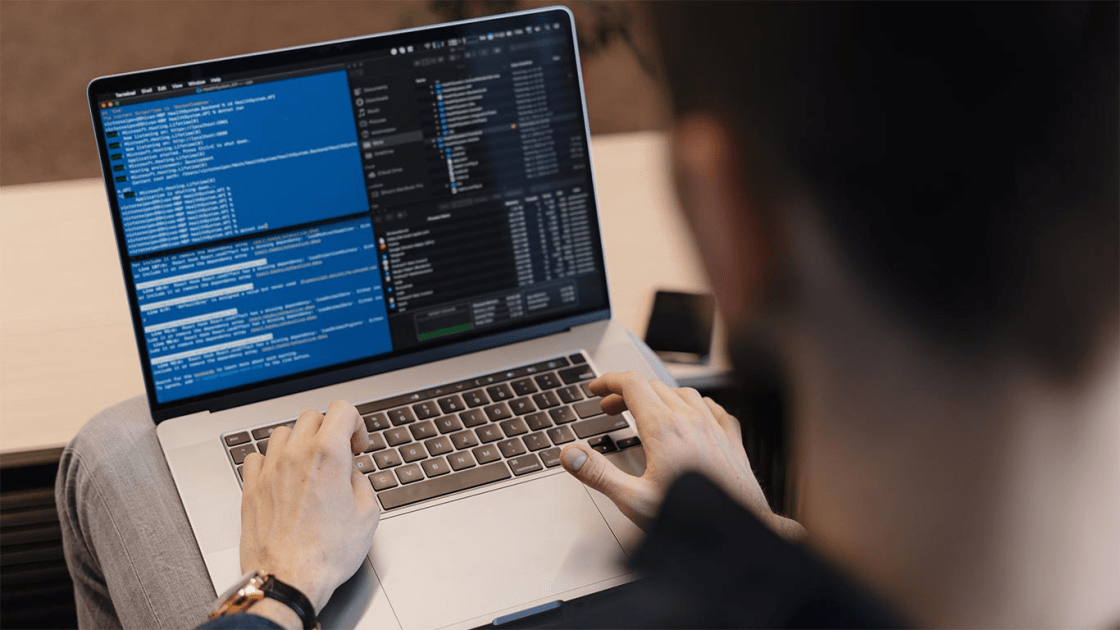
\includegraphics[width=8.92cm,height=5.01cm]{figure/dokumentasi-kegiatan.png}
  \caption{Contoh deskripsi kegiatan}
\end{figure}

\begin{enumerate}[leftmargin=0.635cm,labelwidth=0.635cm,labelsep=0pt,align=left,resume]
  \item \textbf{Minggu 2 (<Tanggal>-<Bulan>-<Tahun>)}
\end{enumerate}


\end{document}
